%%%%%%%%%%%%%%%%%%%%%%%%%%%%%%%%%%%%%%%%%%%%%%%%%%%%%%%%%%%%
%%%%%%%%%%%%%%%%%%%%%%%%%%%%%%%%%%%%%%%%%%%%%%%%%%%%%%%%%%%%
%%%%%%%%%%%%%%%%%%%%%%%%%%%%%%%%%%%%%%%%%%%%%%%%%%%%%%%%%%%%
\section{Finite-dimensional Function Spaces}\label{Sec:General}
%%%%%%%%%%%%%%%%%%%%%%%%%%%%%%%%%%%%%%%%%%%%%%%%%%%%%%%%%%%%
%%%%%%%%%%%%%%%%%%%%%%%%%%%%%%%%%%%%%%%%%%%%%%%%%%%%%%%%%%%%
%%%%%%%%%%%%%%%%%%%%%%%%%%%%%%%%%%%%%%%%%%%%%%%%%%%%%%%%%%%%

Our general PDE problem includes the definition of unconstrained and
constrained finite-dimensional (i.~e.~discrete) function spaces. In
this section we will define such spaces in a general way. 

\subsection{Unconstrained Spaces}

\begin{frame}
\frametitle<presentation>{Finite-dimensional Function Spaces}
$\Omega\subset\mathbb{R}^n$, $n\geq 1$, is a domain, 
$\mathbb{T}_h$ a grid partitioning the domain $\Omega$.

\begin{Def}[Finite-dimensional function space]\label{Def:Vh}
\begin{equation*}\label{Eq:GenericFESpace}
\begin{split}
U_h(\mathbb{T}_h) &= \Biggl\{ u_h(x) : \bigcup_{e\in E_h^0}\Omega_e
 \to \mathbb{K}^m\,\Bigg| \\
&\quad u_h(x) = \sum_{e\in E_h^0}\sum_{i=0}^{k(e)-1} (\mathbf{u})_{g(e,i)}
\, \pi_e(\hat{x}) \, \hat\phi_{e,i}(\hat{x}) \, \chi_e(x); \, \hat{x}=\mu_e^{-1}(x) 
 \Biggr\}
\end{split}
\end{equation*}
defines a general finite-dimensional function space of element-wise
continuous functions.\hfill$\square$ 
\end{Def}
\end{frame}

The individual components in this definition are:
\begin{frame}<article>
\frametitle<presentation>{Finite-dimensional Function Spaces (Contd.)}
\begin{itemize}
\item $\mathbb{K}=\mathbb{R}$ or $\mathbb{K}=\mathbb{C}$.
  $m\geq 1$ denotes vector-valued function spaces. 
\item $\hat\Omega_e$ is the \textit{reference element} associated with
element $e\in E_h^0$. $\mu_e : \overline{\hat\Omega}_e \to
  \overline{\Omega}_e$ maps the reference element to $\Omega$.
\item $\hat\Phi_e
  = \left\{\hat\phi_{e,i}: \overline{\hat\Omega}_e \to \mathbb{R}^{m'}\,|\,0\leq
  i < k(e)\right\}$ is 
  the set of \textit{local basis functions} for element $e$.
\item $\pi_e(\hat{x})\in\mathbb{R}^{m\times m'}$ is a
  transformation. A non-trivial example is the Piola
  transformation \cite{BrezziFortin}
\begin{equation*}
\pi_e(\hat{x}) = \frac{1}{\text{det}\  \nabla\mu_e(\hat{x})} \nabla \mu_e(\hat{x})
\end{equation*}
where $\nabla \mu_e$ denotes the Jacobian of the map $\mu_e$. For most
finite element spaces $\pi_e$ is just the identity and we have $m'=m$.
\item $g : L \to \mathbb{N}$, $L=\left\{ (e,i)\in E_h^0 \times
  \mathbb{N} \,|\, 0\leq i < k(e)\right\}$ is the \textit{local to global map}
  and $\mathcal{I}_{U_h} = \text{im}\,g$ is the associated \textit{global index set}.
\item $\mathbf{u}\in \mathbf{U}=\mathbb{K}^{\mathcal{I}_{U_h}}$ is a coefficient vector.
\end{itemize}
\end{frame}

\begin{frame}
\frametitle<presentation>{Global Basis}
For $j\in \mathcal{I}_{U_h}$ we define the \textit{global basis function}
\begin{equation*}
U_h \ni \phi_j(x) = \sum_{(e,i)\in l(j)} \pi_e(\mu_e^{-1}(x)) \,
\hat\phi_{e,i}(\mu_e^{-1}(x)) \, \chi_e(x)
\end{equation*} 
and $l(j) = \left\{ (e,i)\in L \,|\, g(e,i)=j \right\}$.
With that we have
\begin{align}
\Phi_{U_h} &= \{\phi_i \,|\, i\in \mathcal{I}_{U_h}\}, & U_h &= \text{span}\ \Phi_{U_h}.
\end{align}
and the finite element isomorphism
\begin{align}\label{Eq:FiniteElementIsomorphism}
\text{FE}_{\Phi_{U_h}} &: \mathbf{U} \to
U_h, & \text{FE}_{\Phi_{U_h}}(\mathbf{u})
&= \sum_{i\in\mathcal{I}_{U_h}} (\mathbf{u})_i \phi_i \ . 
\end{align} 

Definition \ref{Def:Vh} allows for functions that are
\textit{discontinuous} at element boundaries. 

If limits on the skeleton $\Gamma_h = \Omega\setminus \bigcup_ {e\in
  E_h^0} \Omega_e$ coincide, a function may be extended to 
$\left(C^0(\Omega)\right)^m$.
\end{frame}

\subsection{Constrained Spaces}

As we have seen we often have the situation that problems have to be solved in a
subspace $\tilde{U}_h\subset U_h$ or even an affine subspace
$w_h+\tilde{U}_h$, where $w_h\in U_h$.

\paragraph{Basis transformation} 

\begin{frame}
\frametitle<presentation>{Basis Transformation}
\begin{Def}[Basis Transformation] Consider an alternative basis
$\Phi_{U_h}'=\{\phi_i'\,|\, i\in \mathcal{I}_{U_h}\}$ of $U_h$
obtained by
\begin{equation}
\phi_i' = \sum_{j\in\mathcal{I}_{U_h}}
\left(\mathbf{T}_{U_h}\right)_{i,j} \phi_j, \qquad i\in \mathcal{I}_{U_h}.
\end{equation}
$\mathbf{T}_{U_h}$ is the \textit{transformation matrix}.\hfill$\square$
\end{Def}
For $\mathbf{U}'=\mathbb{K}^{\mathcal{I}_{U_h}}$ we have the isomorphism
$\text{FE}_{\Phi_{U_h}'}(\mathbf{u}') = \sum_{i\in\mathcal{I}_{U_h}}
(\mathbf{u}')_i \phi_i'$ and get
\begin{equation}
\begin{split}
u_h &= \text{FE}_{\Phi_{U_h}'}(\mathbf{u}') = 
\sum_{j\in\mathcal{I}_{\tilde{U}_h}} (\mathbf{u}')_j \phi'_j = 
\sum_{j\in\mathcal{I}_{U_h}} (\mathbf{u}')_j \left (
\sum_{i\in\mathcal{I}_{U_h}}
\left(\mathbf{T}_{U_h}\right)_{j,i} \phi_i \right)\\
&= \sum_{i\in \mathcal{I}_{U_h}} \left (\sum_{j\in\mathcal{I}_{U_h}}
\left(\mathbf{T}^T_{U_h}\right)_{i,j} (\mathbf{u}')_j \right ) \phi_i
= \text{FE}_{\Phi_{U_h}}\left( \mathbf{T}^T_{U_h} \mathbf{u}' \right) .
\end{split}
\end{equation}
\end{frame}

\paragraph{Splitting and Subspaces} 

\begin{frame}
\frametitle<presentation>{Splitting and Subspaces}
Subspaces are introduced by a splitting of
the index set into unconstrained and constrained indices:
\begin{equation*}
\mathcal{I}_{U_h} = \tilde{\mathcal{I}}_{U_h} \cup
\bar{\mathcal{I}}_{U_h}, \qquad  \tilde{\mathcal{I}}_{U_h} \cap
\bar{\mathcal{I}}_{U_h} = \emptyset.
\end{equation*}
With respect to this splitting we define the subspaces
\begin{align*}
\tilde{U}_h' &= \text{span}\ \{\phi_i'\,|\,
i\in\tilde{\mathcal{I}}_{U_h}\}, &
\bar{U}_h' &= \text{span}\ \{\phi_i'\,|\,
i\in\bar{\mathcal{I}}_{U_h}\}
\end{align*}
and the corresponding coefficient spaces
\begin{align*}
\tilde{\mathbf{U}}' &=
\mathbb{K}^{\tilde{\mathcal{I}}_{U_h}}, &
\bar{\mathbf{U}}' &=
\mathbb{K}^{\bar{\mathcal{I}}_{U_h}}.
\end{align*}

$\tilde{U}_h := \tilde{U}_h'\subseteq U_h$ is the desired subspace of
$U_h$ where we want to solve the constrained problem.
\end{frame}


\begin{frame}
\frametitle<presentation>{Simplified Transformation Matrix}
The transformation matrix $\mathbf{T}_{U_h}$ is written in block
form w.r.t. the splitting:
\begin{equation*}
\mathbf{T}_{U_h} = \left(\begin{array}{cc}
\mathbf{T}_{\tilde{U}_h,\tilde{U}_h} & \mathbf{T}_{\tilde{U}_h,\bar{U}_h}\\
\mathbf{T}_{\bar{U}_h,\tilde{U}_h} & \mathbf{T}_{\bar{U}_h,\bar{U}_h}
\end{array}\right) .
\end{equation*}
We show below that it suffices to consider transformations of the form
\begin{equation}\label{Eq:StructureTransformation}
\mathbf{T}_{U_h} = \left(\begin{array}{cc}
\mathbf{I} & \mathbf{T}_{\tilde{U}_h,\bar{U}_h}\\
\mathbf{0} & \mathbf{I}
\end{array}\right)
\end{equation}
which means transformations have the form
\begin{equation*}
\phi_i' = \phi_i + \sum_{j\in\bar{\mathcal{I}}_{U_h}}
\left(\mathbf{T}_{\tilde{U}_h,\bar{U}_h}\right)_{i,j} \phi_j, \qquad i\in \tilde{\mathcal{I}}_{U_h}.
\end{equation*}
The $\tilde{\mathcal{I}}_{U_h} \times \bar{\mathcal{I}}_{U_h}$  matrix
$\mathbf{T}_{\tilde{U}_h,\bar{U}_h}$ will usually be very sparse (or
even zero).
\end{frame}

\paragraph{Restrictions} 

\begin{frame}<article>
\frametitle<presentation>{Restriction Operators}
Below we will make use of the following restriction operators
\begin{align*}
\mathbf{R}_{\tilde{\mathbf{U}}',\mathbf{U}'} &: \mathbf{U}' \to \tilde{\mathbf{U}}', & 
(\mathbf{R}_{\tilde{\mathbf{U}}',\mathbf{U}'}\mathbf{u}')_i &= 
(\mathbf{u}')_i \quad \forall i\in \tilde{\mathcal{I}}_{U_h},\\
\mathbf{R}_{\bar{\mathbf{U}}',\mathbf{U}'} &: \mathbf{U}' \to \bar{\mathbf{U}}', & 
(\mathbf{R}_{\bar{\mathbf{U}}',\mathbf{U}'}\mathbf{u}')_i &= 
(\mathbf{u}')_i \quad \forall i\in \bar{\mathcal{I}}_{U_h}.
\end{align*}

Note that $\mathbf{Q}_{\tilde{\mathbf{U}}}
= \mathbf{R}_{\tilde{\mathbf{U}}',\mathbf{U}'}^T \mathbf{R}_{\tilde{\mathbf{U}}',\mathbf{U}'}$
is an orthogonal projection.

It can be used to project a function from $U_h$ to $\tilde{U}_h$ as
follows:
\begin{align*}
P_h &: U_h \to \tilde{U}_h, & P_h  =
FE_{\Phi_h'} \circ \mathbf{Q}_{\tilde{\mathbf{U}}} \circ
FE_{\Phi_h'}^{-1} .
\end{align*}

The projection $P_h$ will play a major role below.
\end{frame}

\subsection{Examples of Constrained Spaces}

\paragraph{Dirichlet Boundary Conditions}

\begin{frame}
\frametitle<presentation>{Dirichlet Boundary Conditions}
$U_h^1$ :  piecewise-linear, conforming finite
element functions.

$\tilde{U}_h^1 = \{u\in U_h^1 \,|\, \text{``$u(x)=0$'' for
$x\in \Gamma_D$}\}$.

Then just set 
\begin{align*}
\bar{\mathcal{I}}_{U_h} &= \{i\in \mathcal{I}_{U_h} \,|\,
x_{z_i}\in\Gamma_D\}, &
\tilde{\mathcal{I}}_{U_h} =  \mathcal{I}_{U_h}\setminus\bar{\mathcal{I}}_{U_h}
\end{align*}
and
\begin{equation*}
\phi_i' = \phi_i \qquad i\in \tilde{\mathcal{I}}_{U_h}.
\end{equation*}

Obviously, $\mathbf{T}_{\tilde{U}_h,\bar{U}_h}=\mathbf{0}$ in this case.
\end{frame}

\paragraph{Hanging Nodes}

Consider a mesh obtained from non-conforming refinement.

\begin{frame}
\frametitle<presentation>{Hanging Nodes}
\begin{columns}
\begin{column}{0.6\textwidth}
$U_h^1$ now is the space of piecewise linear functions with degrees of
freedom in \textit{all} vertices of the mesh. \\
\medskip
To obtain the subspace $\tilde{U}_h^1 = U_h^1 \cap C^0(\Omega)$ we set 
\begin{align*}
\bar{\mathcal{I}}_{U_h} &= \{i\in \mathcal{I}_{U_h} \,|\, \text{$z_i$ is a
hanging node} \}, \\
\tilde{\mathcal{I}}_{U_h} &=  \mathcal{I}_{U_h}\setminus\bar{\mathcal{I}}_{U_h}.
\end{align*}
\end{column}
\mode<presentation>{
\begin{column}{0.4\textwidth}
\psfrag{0}{{\tiny $0$}}
\psfrag{1}{{\tiny $1$}}
\psfrag{h}{{\tiny $\frac12$}}
\psfrag{vi}{$v_i$}
\psfrag{vj}{$v_j$}
\psfrag{vk}{$v_k$}
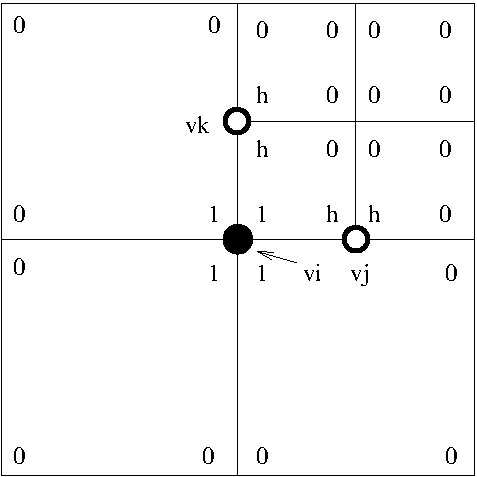
\includegraphics[width=\textwidth]{./EPS/function3}
\end{column}}
\end{columns}
\mode<article>{
\begin{figure}
\begin{center}
\psfrag{0}{{\tiny $0$}}
\psfrag{1}{{\tiny $1$}}
\psfrag{h}{{\tiny $\frac12$}}
\psfrag{vi}{$v_i$}
\psfrag{vj}{$v_j$}
\psfrag{vk}{$v_k$}
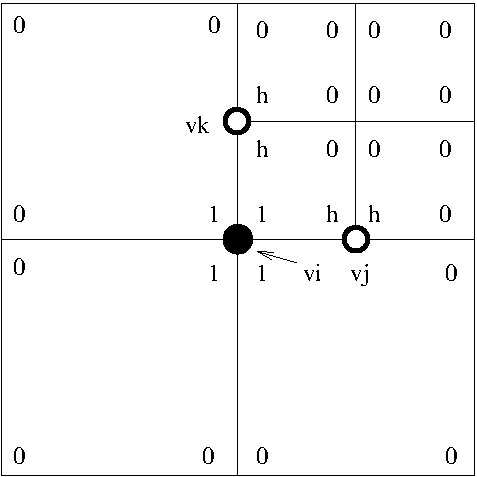
\includegraphics[width=0.5\textwidth]{./EPS/function3}
\end{center}
\caption{Non-conforming refinement and piecewise linear finite elements.}
\end{figure}}
For the vertex $i$ in the figure we obtain, e.~g., the basis function
\begin{equation*}
\phi_i' = \phi_i + \frac12 \phi_j + \frac12 \phi_k .
\end{equation*}
\end{frame}


\paragraph{Pure Neumann Problem}

\begin{frame}<article>
\frametitle<presentation>{Pure Neumann Problem}
We wish to solve
\begin{align*}
                -\Delta u &= f& \text{in }& \Omega\subseteq\mathbb{R}^n,\\
     - \nabla u\cdot\nu   &= j& \text{on }& \partial\Omega
\end{align*}
where $\int_{\partial\Omega} j \, ds = \int_\Omega f \, dx$.

Again, consider $U_h^1$, the piecewise-linear, conforming finite
element functions.

Then $u$ is only defined up to a constant and we wish to solve in
\begin{equation*}
\tilde{U}^1_h = \left\{u \in U^1_h \,\Biggl |\, \int_\Omega u \, dx = 0\right\}.
\end{equation*}

Set $\bar{\mathcal{I}}_{U_h}=\{0\}$, $\tilde{\mathcal{I}}_{U_h}
= \mathcal{I}_{U_h}\setminus\{0\}$ and
\begin{equation*}
\phi_i' = \phi_i - \frac{\int_\Omega\phi_i\, dx}{\int_\Omega\phi_0\,
dx} \phi_0, \qquad \forall i\in\tilde{\mathcal{I}}_{U_h}.
\end{equation*}
\end{frame}

\paragraph{Other Situations Where Constraints Occur}

\begin{frame}
\frametitle<presentation>{Other Constraints}
In addition to Dirichlet, hanging nodes and pure Neumann constraints we can also treat
\begin{itemize}
\item Varying polynomial degree in conforming finite elements
($p$-refinement).
\item Combination of $p$-refinement, non-conforming refinement and essential
boundary conditions.
\item Non-conforming refinement in mixed finite elements.
\item Periodic boundary conditions.
\item Constraints in parallel overlapping Schwarz methods.
\end{itemize}
\end{frame}


\subsection{Function Space Composition}

\begin{frame}
\frametitle<presentation>{Function Space Composition}
For systems we need composite function spaces.

Given $k>1$ function spaces $U_0, \ldots, U_{k-1}$ we define the
composite function space 
\begin{equation}
U = U_0 \times U_1 \times \ldots \times U_{k-1} .
\end{equation}

If all component spaces are the same we can also write
\begin{equation}
U = V^k
\end{equation}

This can be done recursively. E.g. for solving the Stokes equation
in dimension $d$ using Taylor-Hood elements we would require
\begin{equation*}
U_h^\text{TH} = \left( U_h^2\right)^d \times U_h^1
\end{equation*}

Composite function spaces can be visualized as a tree:
\begin{minipage}[c]{0.2\textwidth}
\psfrag{P1}{$U_h^1$} 
\psfrag{P2}{$U_h^2$} 
\psfrag{TH}{$U_h^\text{TH}$} 
\psfrag{Vel}{$U_h^\text{V}$} 
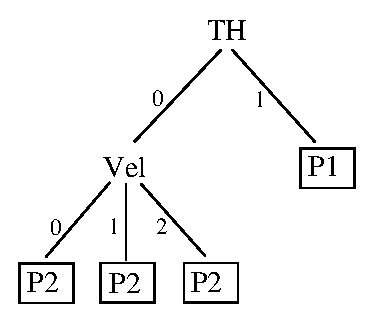
\includegraphics[width=\textwidth]{./EPS/THBaum}
\end{minipage}

\end{frame}

\cleardoublepage

%%%%%%%%%%%%%%%%%%%%%%%%%%%%%%%%%%%%%%%%%%%%%%%%%%%%%%%%%%%%
%%%%%%%%%%%%%%%%%%%%%%%%%%%%%%%%%%%%%%%%%%%%%%%%%%%%%%%%%%%%
%%%%%%%%%%%%%%%%%%%%%%%%%%%%%%%%%%%%%%%%%%%%%%%%%%%%%%%%%%%%
\section{Discrete Functions in \texttt{dune-pdelab}}
%%%%%%%%%%%%%%%%%%%%%%%%%%%%%%%%%%%%%%%%%%%%%%%%%%%%%%%%%%%%
%%%%%%%%%%%%%%%%%%%%%%%%%%%%%%%%%%%%%%%%%%%%%%%%%%%%%%%%%%%%
%%%%%%%%%%%%%%%%%%%%%%%%%%%%%%%%%%%%%%%%%%%%%%%%%%%%%%%%%%%%

\subsection{Local Finite Element Space}

A global finite element space is built up from a collection of local
finite element spaces for each element.

\begin{frame}
\frametitle<presentation>{Local Finite Element Space}
A local finite element space (compare \cite{Ciarlet}) 
is represented by \lstinline{Dune::LocalFiniteElementInterface}
and consists of the following:
\begin{itemize}
\item The type of reference element, given by \lstinline{Dune::GeometryType}.
\item The local basis functions
$\hat\Phi = \{\hat\phi_i : \mathbb{D}^n \to \mathbb{K}^m \,|\, 0\leq i < k\}$
and their gradients in a class derived from \lstinline{Dune::C1LocalBasisInterface}.
\item Information that allows to construct the local to global map $g:
(e,i) \mapsto j$ in a class derived
from \lstinline{Dune::LocalCoefficientsInterface}. 
\item A method that allows to compute coefficients $z_i$ such that
\begin{equation*}
\sum_{0\leq i < k} z_i \hat\phi_i = \hat{u} \qquad \hat{u}\in\text{span}\hat\Phi 
\end{equation*} 
in a class derived
from \lstinline{Dune::LocalInterpolationInterface}. For
$\hat{u}\not\in\text{span}\hat\Phi$ the method provides a projection.
\item The dune module \lstinline{dune-localfunctions} provides a
collection of local finite element spaces.
\end{itemize}
\end{frame}

\begin{frame}[fragile]
\frametitle<presentation>{Function Traits}
The local basis is required to contain a class \lstinline{Traits} that
gives the types for
$\mathbb{D}, \mathbb{D}^n, \mathbb{K}, \mathbb{K}^m$, the numbers $n$,
$m$ and a type for the Jacobian:
\begin{lstlisting}[basicstyle=\ttfamily\scriptsize,numbers=left, 
numberstyle=\tiny, numbersep=5pt]
template<class DF, int n, class D, class RF, int m, class R>
struct C0LocalBasisTraits 
{
  typedef DF DomainFieldType; typedef D DomainType;
  typedef RF RangeFieldType;  typedef R RangeType;
  enum { dimDomain=n }; enum { dimRange=m }; enum { diffOrder=0 };
};
\end{lstlisting}
\begin{lstlisting}[basicstyle=\ttfamily\scriptsize,numbers=left, 
numberstyle=\tiny, numbersep=5pt]
template<class DF, int n, class D, class RF, int m, class R, class J>
struct C1LocalBasisTraits : public C0LocalBasisTraits<DF,n,D,RF,m,R> 
{
  typedef J JacobianType; enum { diffOrder=1 };
};
\end{lstlisting}

Note: Basis functions may be vector-valued.

Later on, other classes representing functions will use the same
traits classes.
\end{frame}

\begin{frame}
\frametitle<presentation>{$Q_1$ Local Basis}
We now consider the bilinear elements $Q_1$ as an example.

The basis functions are given by
\begin{align*}
\hat\phi_2(\hat{x}) &= (1-\hat{x}_0)\hat{x}_1, &
\hat\phi_3(\hat{x}) &= \hat{x}_0\hat{x}_1, \\
\hat\phi_0(\hat{x}) &= (1-\hat{x}_0)(1-\hat{x}_1), &
\hat\phi_1(\hat{x}) &= \hat{x}_0(1-\hat{x}_1).
\end{align*}


\begin{columns}
\begin{column}{0.65\textwidth}
The numbering of the basis functions corresponds to the reference
quadrilateral.
\end{column}
\mode<presentation>{
\begin{column}{0.3\textwidth}
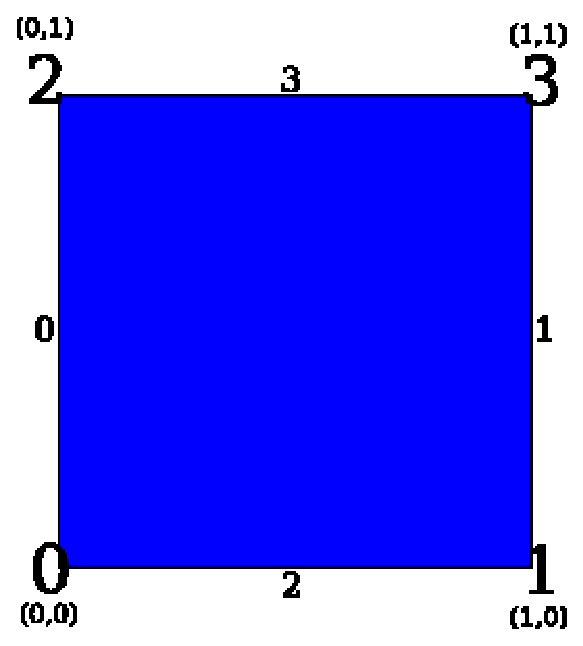
\includegraphics[width=\textwidth]{./EPS/quadrilateral}
\end{column}}
\end{columns}

\mode<article>{
\begin{figure}
\begin{center}
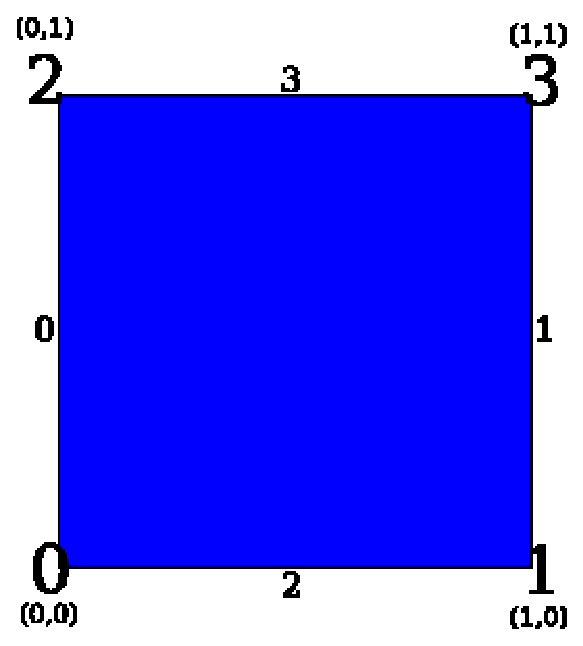
\includegraphics[width=0.5\textwidth]{./EPS/quadrilateral}
\end{center}
\caption{DUNE reference quadrilateral.}
\end{figure}}
\end{frame}

\begin{frame}[fragile]
\frametitle<presentation>{$Q_1$ Local Basis Implementation}
The following listing gives an implementation of the local basis
functions. 

The base class \lstinline{Dune::C1LocalBasisInterface} provides
provides a Barton-Nackman style interface base class for
differentiable basis functions.

This interface will be extended to provide also higher derivatives.

There is also an interface \lstinline{Dune::C0LocalBasisInterface}
when no derivatives are provided.

Evaluation always provides the values of \textit{all} basis functions
or gradients at \textit{one} point. 

Implementations typically use \lstinline{Dune::FieldVector<T,n>} to
represent short vectors.

\lstinline{JacobianType} is \lstinline{Dune::FieldVector<Dune::FieldVector<R,2>,1>}.

In the jacobian evaluation in lines \ref{q1b:grad0} to \ref{q1b:grad3}
we have
\begin{equation*}
\text{\lstinline{out[i][j][k]}}
= \partial_{\hat{x}_k} \left(\hat\phi_i\right)_j (\hat{x}) . 
\end{equation*}
\end{frame}


\begin{frame}<presentation>[fragile,allowframebreaks,allowdisplaybreaks]
\frametitle<presentation>{$Q_1$ Local Basis Listing}
\framesubtitle<presentation>{File \texttt{examples/q1localbasis.hh}}
\lstinputlisting[basicstyle=\ttfamily\scriptsize,numbers=left, 
numberstyle=\tiny, numbersep=5pt]{../../examples/q1localbasis.hh}
\end{frame}
\mode<article>{
\begin{Lst}[File examples/q1localbasis.hh] \mbox
\nopagebreak
\lstinputlisting[basicstyle=\ttfamily\scriptsize,numbers=left, 
numberstyle=\tiny, numbersep=5pt]{../../examples/q1localbasis.hh}
\end{Lst}}


\begin{frame}
\frametitle<presentation>{$Q_1$ Local Coefficients}
In order to provide (different forms of) continuity of \textit{global} basis
functions local indices in \textit{adjacent} elements need to be \textit{identified}.

This is done via (sub-)entities of a given codim 0 entity.

\textit{On the reference element} each local index $0\leq i < k$ is
mapped to
\begin{itemize}
\item a subentity given by a number and a codimension.
\item an offset with in that entity if several indices are mapped to
the same subentity (offset is zero if only one local index is mapped
to the subentity). 
\end{itemize} 

From this information a local-to-global map $g$ can be
constructed \textit{generically}. 

Class \lstinline{Dune::LocalKey} collects subentity and offset information.

For the $Q_1$ element the code is given by the following listing.
\end{frame}

\begin{frame}<presentation>[fragile,allowframebreaks,allowdisplaybreaks]
\frametitle<presentation>{$Q_1$ Local Coefficients Listing}
\framesubtitle<presentation>{File \texttt{examples/q1localcoefficients.hh}}
\lstinputlisting[basicstyle=\ttfamily\scriptsize,numbers=left, 
numberstyle=\tiny, numbersep=5pt]{../../examples/q1localcoefficients.hh}
\end{frame}
\mode<article>{
\begin{Lst}[File examples/q1localcoefficients.hh] \mbox
\nopagebreak
\lstinputlisting[basicstyle=\ttfamily\scriptsize,numbers=left, 
numberstyle=\tiny, numbersep=5pt]{../../examples/q1localcoefficients.hh}
\end{Lst}}


\begin{frame}
\frametitle<presentation>{$Q_1$ Local Interpolation}
Local interpolation takes a function $\hat{u}(\hat{x})$ \textit{on the
reference element} and provides a projection onto the space spanned by
the local basis.

For Lagrange basis functions this is point-wise evaluation.

For other basis functions this might involve the solution of a local
system (e.g. $L_2$-projection).

The local interpolation interface is provided by
\lstinline{Dune::LocalInterpolationInterface}.
\end{frame}


\begin{frame}<presentation>[fragile,allowframebreaks,allowdisplaybreaks]
\frametitle<presentation>{$Q_1$ Local Interpolation Listing}
\framesubtitle<presentation>{File \texttt{examples/q1localinterpolation.hh}}
\lstinputlisting[basicstyle=\ttfamily\scriptsize,numbers=left, 
numberstyle=\tiny, numbersep=5pt]{../../examples/q1localinterpolation.hh}
\end{frame}
\mode<article>{
\begin{Lst}[File examples/q1localinterpolation.hh] \mbox
\nopagebreak
\lstinputlisting[basicstyle=\ttfamily\scriptsize,numbers=left, 
numberstyle=\tiny, numbersep=5pt]{../../examples/q1localinterpolation.hh}
\end{Lst}}

\begin{frame}
\frametitle<presentation>{$Q_1$ Local Finite Element}
Finally, we need to collect local basis, local coefficients and local
interpolation in a local finite element.

Local finite element also provides the reference element.

The interface is given
in \lstinline{Dune::LocalFiniteElementInterface}.

Currently (March 2009), \lstinline{dune-localfunctions} implements the
following elements:
\begin{itemize}
\item Piecewise constant elements $P_0$ for any reference element in any
dimension. 
\item Piecewise linear Lagrange elements $P_1$ in $1, 2, 3d$.
\item Piecewise multi-linear Lagrange elements $Q_1$ in $1, 2, 3d$.
\item $P_k$ on triangles.
\item $Q_2$ on quadrilaterals.
\item Lowest order Raviart-Thomas elements on triangles. 
\end{itemize}
\end{frame}

\begin{frame}<presentation>[fragile,allowframebreaks,allowdisplaybreaks]
\frametitle<presentation>{$Q_1$ Local Finite Element Listing}
\framesubtitle<presentation>{File \texttt{examples/q1localfiniteelement.hh}}
\lstinputlisting[basicstyle=\ttfamily\scriptsize,numbers=left, 
numberstyle=\tiny, numbersep=5pt]{../../examples/q1localfiniteelement.hh}
\end{frame}
\mode<article>{
\begin{Lst}[File examples/q1localfiniteelement.hh] \mbox
\nopagebreak
\lstinputlisting[basicstyle=\ttfamily\scriptsize,numbers=left, 
numberstyle=\tiny, numbersep=5pt]{../../examples/q1localfiniteelement.hh}
\end{Lst}}


\subsection{Unconstrained Global Finite Element Space}

\begin{frame}
\frametitle<presentation>{Local Finite Element Map}
A global finite element space is made up from a collection of local
finite element spaces. 

So we need a map that delivers for each element (codim 0 entity) $e\in E_h^0$ a
local finite element.

But there is only one \textit{type} for all the local finite elements in the map.
This type may be polymorphic if needed.

For multi-element type meshes and $hp$-refinement this map may be
rather complicated.

In our implementation of $P_k$ elements for $k>2$ we use the map to
match the degrees of freedom on common edges and faces.

For the special case where we have \textit{the same} local finite
element for \textit{all} the elements there is a default implementation that is
used in the following listing.
\end{frame}

\begin{frame}<presentation>[fragile,allowframebreaks,allowdisplaybreaks]
\frametitle<presentation>{$Q_1$ Local Finite Element Map Listing}
\framesubtitle<presentation>{File \texttt{examples/q1localfiniteelementmap.hh}}
\lstinputlisting[basicstyle=\ttfamily\scriptsize,numbers=left, 
numberstyle=\tiny, numbersep=5pt]{../../examples/q1localfiniteelementmap.hh}
\end{frame}
\mode<article>{
\begin{Lst}[File examples/q1localfiniteelementmap.hh] \mbox
\nopagebreak
\lstinputlisting[basicstyle=\ttfamily\scriptsize,numbers=left, 
numberstyle=\tiny, numbersep=5pt]{../../examples/q1localfiniteelementmap.hh}
\end{Lst}}


\begin{frame}
\frametitle<presentation>{$Q_1$ Grid Function Space}
Now we use the $Q_1$ local finite element map to build
a global finite element space.

The main class is \lstinline{GridFunctionSpace} which 
builds up the local to global map $g$ and provides information about
the local finite elements.

An element of the function space is represented by a coefficient
vector that is
encapsulated in a seperate type, see definition \lstinline{X}.

The type \lstinline{X} is derived from \lstinline{std::vector<R>} here
but his will be changed later.

The remaining lines construct a function object that can be evaluated
in local coordinates on the reference element (explained below).

\lstinline{Dune::SubsamplingVTKWriter} allows the output of
nonconforming and higher order functions.
\end{frame}

\begin{frame}<presentation>[fragile,allowframebreaks,allowdisplaybreaks]
\frametitle<presentation>{$Q_1$ Grid Function Space Listing}
\framesubtitle<presentation>{File \texttt{examples/q1gridfunctionspace.hh}}
\lstinputlisting[basicstyle=\ttfamily\scriptsize,numbers=left, 
numberstyle=\tiny, numbersep=5pt]{../../examples/q1gridfunctionspace.hh}
\end{frame}
\mode<article>{
\begin{Lst}[File examples/q1gridfunctionspace.hh] \mbox
\nopagebreak
\lstinputlisting[basicstyle=\ttfamily\scriptsize,numbers=left, 
numberstyle=\tiny, numbersep=5pt]{../../examples/q1gridfunctionspace.hh}
\end{Lst}}

\begin{frame}
\frametitle<presentation>{$Q_1$ Grid Function Space Main Program}
Finally, in the main program a \lstinline{Dune::Grid} is instantiated
and the generic function is called.

We show only one main program here for illustration. In the other
examples below the main programs will not be listed.
\end{frame}

\begin{frame}<presentation>[fragile,allowframebreaks,allowdisplaybreaks]
\frametitle<presentation>{$Q_1$ GFS Main Program Listing}
\framesubtitle<presentation>{File \texttt{examples/q1gridfunctionspacemain.cc}}
\lstinputlisting[basicstyle=\ttfamily\scriptsize,numbers=left, 
numberstyle=\tiny, numbersep=5pt]{../../examples/q1gridfunctionspacemain.cc}
\end{frame}
\mode<article>{
\begin{Lst}[File examples/q1gridfunctionspacemain.cc] \mbox
\nopagebreak
\lstinputlisting[basicstyle=\ttfamily\scriptsize,numbers=left, 
numberstyle=\tiny, numbersep=5pt]{../../examples/q1gridfunctionspacemain.cc}
\end{Lst}}


\begin{frame}<presentation>
\frametitle<presentation>{$Q_1$ Global Basis Function Visualization}
\begin{center}
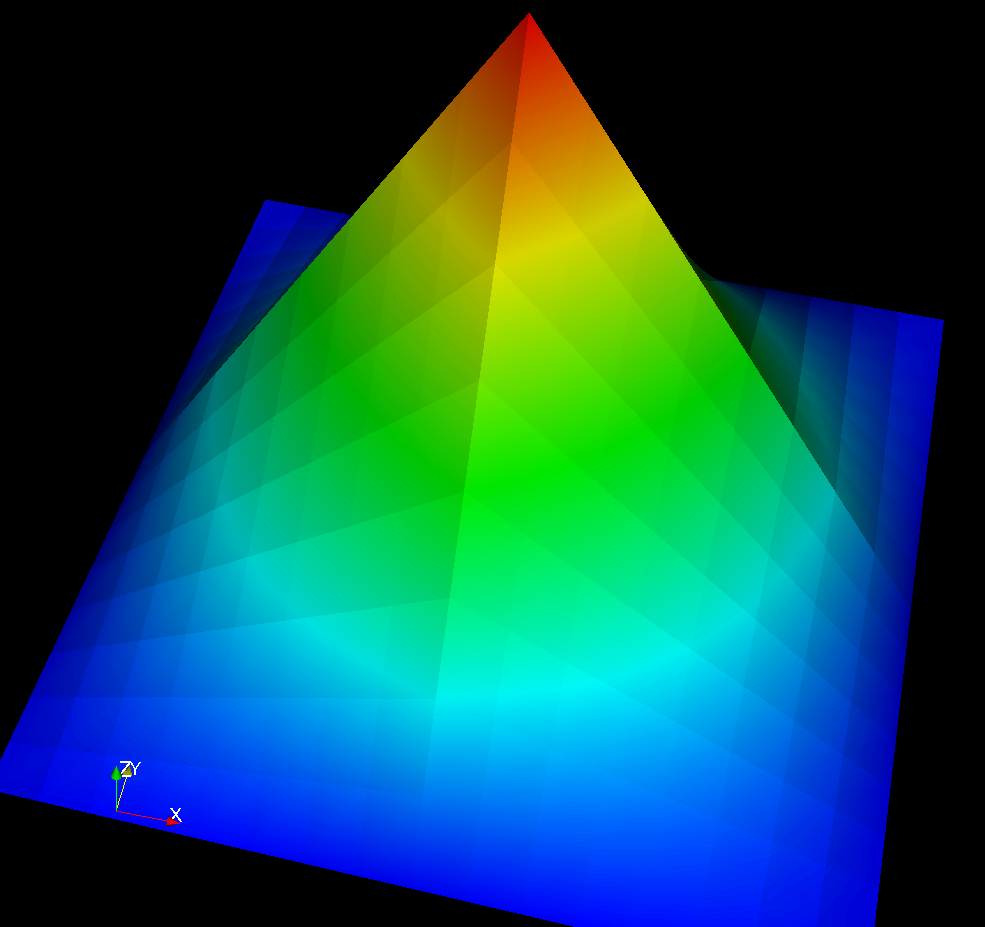
\includegraphics[width=0.65\textwidth]{./EPS/q1}
\end{center}
\end{frame}

Figure \ref{fig:Q1GlobalBasisFunction} shows the result visualized
with ParaView.

\mode<article>{
\begin{figure}
\begin{center}
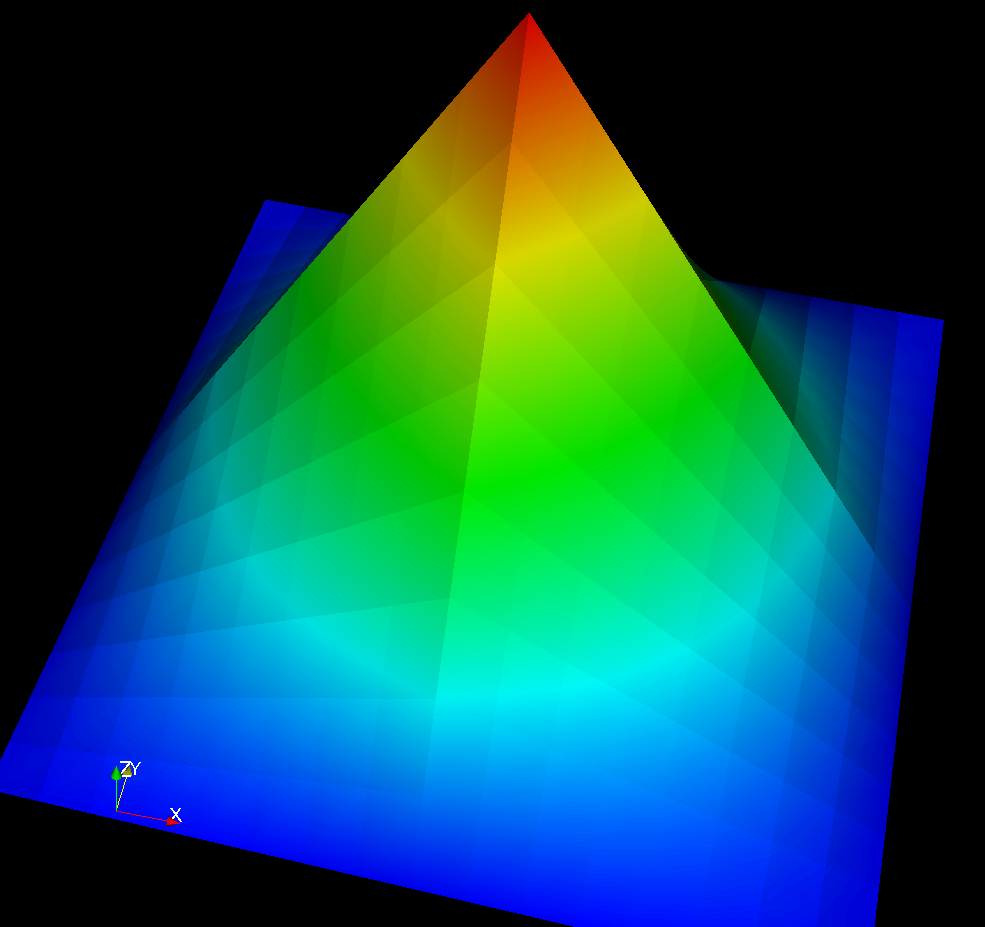
\includegraphics[width=0.5\textwidth]{./EPS/q1}
\end{center}
\caption{$Q_1$ global basis function visualized with ParaView.}
\label{fig:Q1GlobalBasisFunction}
\end{figure}
}

\subsection{Interpolation from Analytic Function}

\mode<article>{
\begin{figure}
\begin{center}
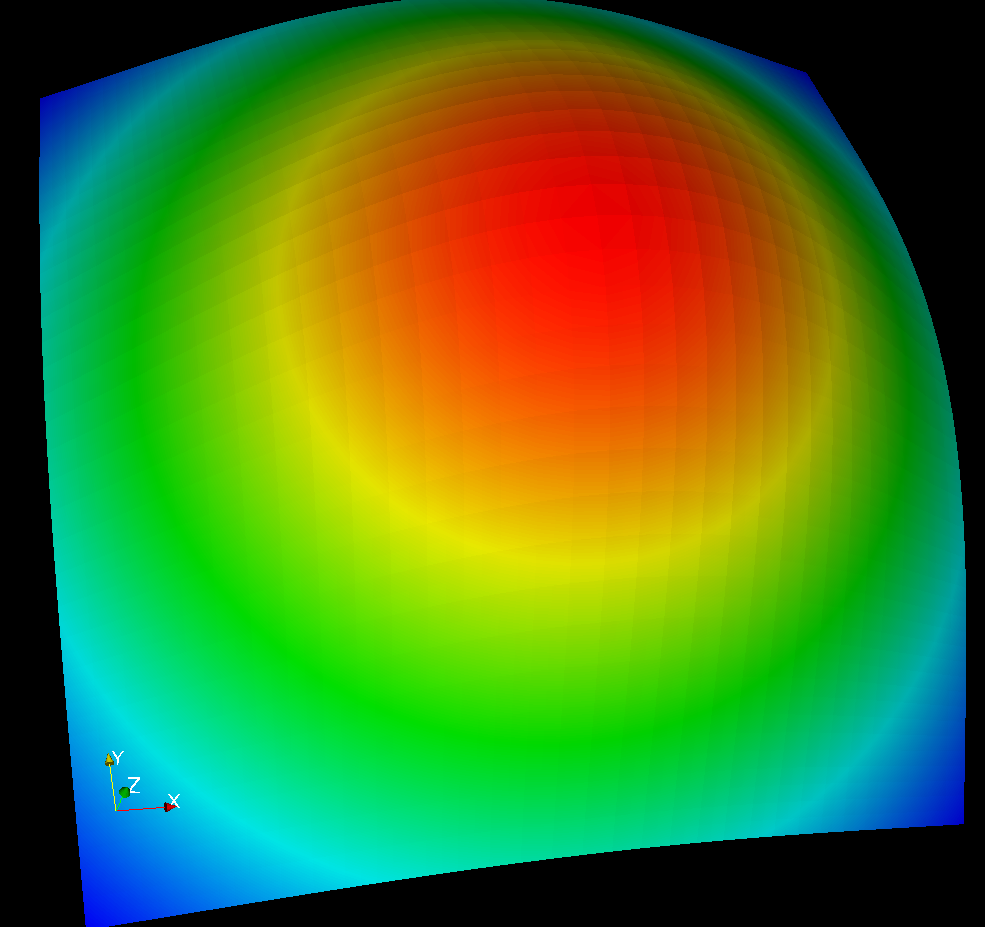
\includegraphics[width=0.5\textwidth]{./EPS/q1interpolate}
\end{center}
\caption{Interpolation of $\exp(-3\|x-c\|^2)$ with $Q_1$ elements.}
\label{fig:Q1Interpolation}
\end{figure}
}

\begin{frame}
\frametitle<presentation>{Functions}
Often one wants to prescribe functions for initial or boundary
conditions.

PDELab offers several classes to represent functions:
\begin{itemize}
\item \lstinline{Dune::PDELab::FunctionInterface} is the interface for general
functions $$u : \mathbb{D}^n \to \mathbb{K}^m, \qquad x \mapsto y.$$ 
\item \lstinline{Dune::PDELab::GridFunctionInterface} is the interface
for functions defined on a grid:
$$u : E_h^0 \times \mathbb{D}^n \to \mathbb{K}^m, \qquad
(e,\hat{x}) \mapsto y.$$
$\hat{x}$ is on the \textit{reference element}.
\item \lstinline{Dune::PDELab::BoundaryGridFunctionInterface} is the
interface for \textit{grid functions} living on the boundary:
$$u : (E_h^1\text{``$\cap\partial\Omega$''}) \times \mathbb{D}^{n'} \to \mathbb{K}^m, \qquad
(f,\hat{x}) \mapsto y.$$
\item Functions offer the same \lstinline{Traits} as the local basis.
\end{itemize}
\end{frame}


\begin{frame}
\frametitle<presentation>{Useful Adapters and Base Classes}
There are various useful adapters and base classes:

\lstinline{Dune::PDELab::DiscreteGridFunction}: Takes a grid
function space and a coefficient vector and makes a grid function out
of it.

\lstinline{Dune::PDELab::VTKGridFunctionAdapter}: Takes a grid
function and makes a VTK function out of it (this is the input
for \lstinline{VTKWriter}). These two classes have been used already above.

\lstinline{Dune::PDELab::AnalyticGridFunctionBase}: Implements
grid function interface from global function by deriving from it.
This class will be used shortly.

\end{frame}

\begin{frame}<article>
\frametitle<presentation>{Less Useful Adapters}
\lstinline{Dune::PDELab::FunctionToGridFunctionAdapter}: Takes a global
function and makes a grid function out of it.

\lstinline{Dune::PDELab::GlobalFunctionToLocalFunctionAdapter}:
Takes a global function and an element and provides evaluation
w.r.t.~reference element.

\lstinline{Dune::PDELab::GridFunctionToLocalFunctionAdapter}:
Takes grid function and element, acts as function on the
reference element.

\lstinline{Dune::PDELab::SelectComponentAdapter}. Takas
vector-valued function and component number and provides a scalar function.

\lstinline{D...::BoundaryGridFunctionSelectComponentAdapter}:
Same for boundary grid functions.

\lstinline{Dune::PDELab::PiolaBackwardAdapter}: Takes global
vector-valued function, makes grid function tranformed back to
reference element.

For more details see \lstinline{dune/pdelab/common/function.hh}.
\end{frame}

\begin{frame}<presentation>[fragile,allowframebreaks,allowdisplaybreaks]
\frametitle<presentation>{\texttt{AnalyticGridFunctionBase} Example Listing}
\framesubtitle<presentation>{File \texttt{examples/analyticfunction.hh}}
\lstinputlisting[basicstyle=\ttfamily\scriptsize,numbers=left, 
numberstyle=\tiny, numbersep=5pt]{../../examples/analyticfunction.hh}
\end{frame}
\mode<article>{
\begin{Lst}[File examples/analyticfunction.hh] \mbox
\nopagebreak
\lstinputlisting[basicstyle=\ttfamily\scriptsize,numbers=left, 
numberstyle=\tiny, numbersep=5pt]{../../examples/analyticfunction.hh}
\end{Lst}}

\begin{frame}
\frametitle<presentation>{Generic Interpolation}
Interpolation of a finite element function from a given function is
now generic.
\end{frame}


\begin{frame}<presentation>[fragile,allowframebreaks,allowdisplaybreaks]
\frametitle<presentation>{Generic Interpolation Listing}
\framesubtitle<presentation>{File \texttt{examples/q1interpolate.hh}}
\lstinputlisting[basicstyle=\ttfamily\scriptsize,numbers=left, 
numberstyle=\tiny, numbersep=5pt]{../../examples/q1interpolate.hh}
\end{frame}
\mode<article>{
\begin{Lst}[File examples/q1interpolate.hh] \mbox
\nopagebreak
\lstinputlisting[basicstyle=\ttfamily\scriptsize,numbers=left, 
numberstyle=\tiny, numbersep=5pt]{../../examples/q1interpolate.hh}
\end{Lst}}

\begin{frame}<presentation>
\frametitle<presentation>{Visualization of the Result}
\begin{center}
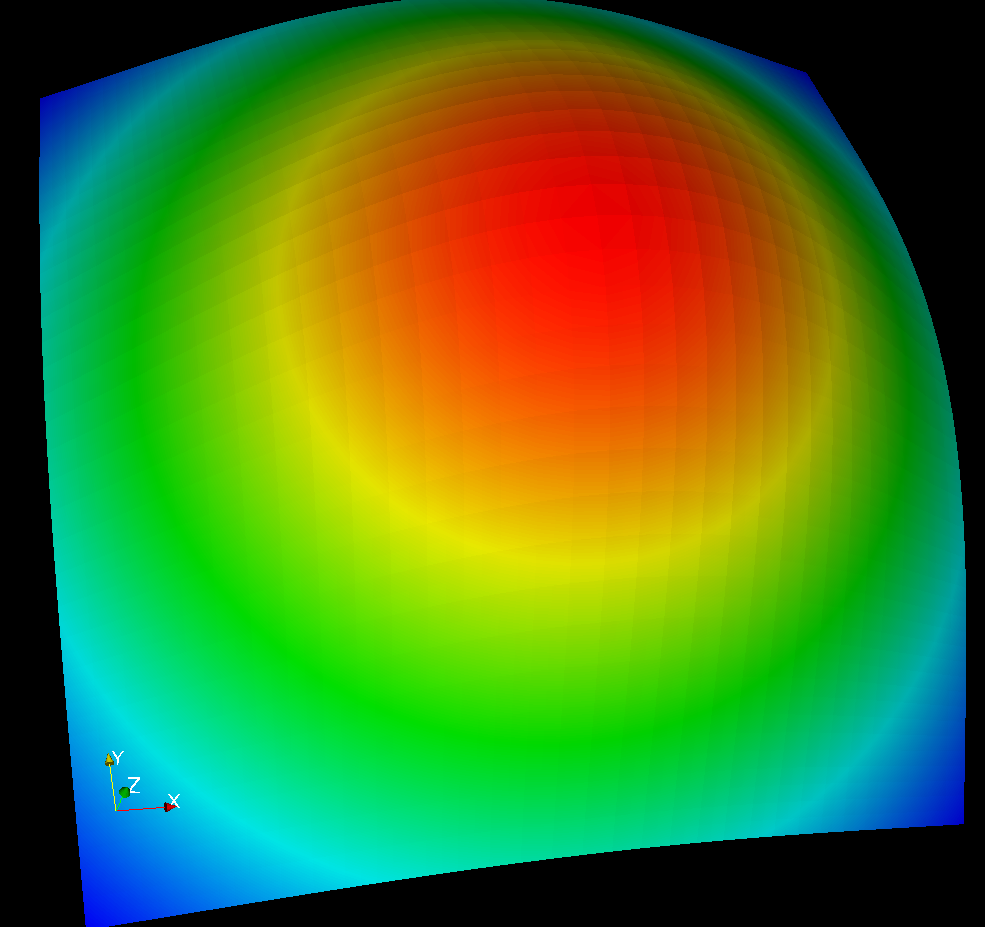
\includegraphics[width=0.65\textwidth]{./EPS/q1interpolate}
\end{center}
\end{frame}



\subsection{Interpolation Error}

\begin{frame}
\frametitle<presentation>{Interpolation Error Example}
Now, we do a little example that shows how one can work with global
finite element functions.

For a given function $u$ and its interpolant $u_h\in
U_h(\mathbb{T}_h)$ we want to compute the $L_2$ interpolation error 
\begin{equation*}
\begin{split}
\|&u-u_h\|_{L_2(\Omega)} = \int_\Omega (u-u_h)^2\, dx 
= \sum_{e\in E_h^0} \int_{\Omega_e} (u-u_h)^2\, dx \\
&= \sum_{e\in E_h^0} \int_{\hat{\Omega}_e} \left(u(\mu_e(\hat{x})) -
u_h(\mu_e(\hat{x})) \right)^2 \text{det} \nabla\mu_e(\hat{x}) \,
d\hat{x}\\
&= \sum_{e\in E_h^0} \sum_{j=0}^{q(e)-1} w_{e,j} \left( u(\mu_e(\hat{x}_{e,j})) -
u_h(\mu_e(\hat{x}_{e,j})) \right)^2 \text{det} \nabla\mu_e(\hat{x}_{e,j}) \,
d\hat{x} \text{ $+$ error}\\
&= \sum_{e\in E_h^0} \sum_{j=0}^{q(e)-1} w_{e,j} \left(u(\mu_e(\hat{x}_{e,j})) -
\sum_{i=0}^{k(e)-1}(\mathbf{u})_{g(e,i)} \hat\phi_{e,i}(\hat{x}_{e,j}) \right)^2  
\text{det} \nabla\mu_e(\hat{x}_{e,j}) \,  
d\hat{x} \text{ $+$ error} .
\end{split}
\end{equation*}
\end{frame}

\begin{frame}
\frametitle<presentation>{Interpolation Error Example}
In the following code example the
function \lstinline{l2interpolationerror} is parametrized by
\begin{itemize}
\item \lstinline{U}: Type for a function. 
\item \lstinline{GFS}: Type for a grid function space.
\item \lstinline{X}: Type for a coefficient vector.
\end{itemize}
The local function space
\lstinline{GFS::LocalFunctionSpace} in line \ref{l2int:lfs} is a type 
exported by a grid function space which
\begin{itemize}
\item is bound to an element $e$ later in line \ref{l2int:bind},
\item provides the local finite element for that element $e$ ,
\item provides the local to global map $g(e,\cdot)$ for that element,
\item can read, write and add degrees of freedom of element $e$.
\end{itemize}
\lstinline{Dune::QuadratureRule} in line \ref{l2int:quad} provides
quadrature rules for many element types, dimensions and orders.
\end{frame}

\begin{frame}<presentation>[fragile,allowframebreaks,allowdisplaybreaks]
\frametitle<presentation>{Interpolation Error Listing}
\framesubtitle<presentation>{File \texttt{examples/l2interpolationerror.hh}}
\lstinputlisting[basicstyle=\ttfamily\scriptsize,numbers=left, 
numberstyle=\tiny, numbersep=5pt]{../../examples/l2interpolationerror.hh}
\end{frame}
\mode<article>{
\begin{Lst}[File examples/l2interpolationerror.hh] \mbox
\nopagebreak
\lstinputlisting[basicstyle=\ttfamily\scriptsize,numbers=left, 
numberstyle=\tiny, numbersep=5pt]{../../examples/l2interpolationerror.hh}
\end{Lst}}

Next comes the driver that uses the generic $L_2$ interpolation error
function.

\begin{frame}<presentation>[fragile,allowframebreaks,allowdisplaybreaks]
\frametitle<presentation>{Interpolation Error Driver Listing}
\framesubtitle<presentation>{File \texttt{examples/q1interpolationerror.hh}}
\lstinputlisting[basicstyle=\ttfamily\scriptsize,numbers=left, 
numberstyle=\tiny, numbersep=5pt]{../../examples/q1interpolationerror.hh}
\end{frame}
\mode<article>{
\begin{Lst}[File examples/q1interpolationerror.hh] \mbox
\nopagebreak
\lstinputlisting[basicstyle=\ttfamily\scriptsize,numbers=left, 
numberstyle=\tiny, numbersep=5pt]{../../examples/q1interpolationerror.hh}
\end{Lst}}

\begin{frame}[fragile]
\frametitle<presentation>{$Q_1$ Interpolation Error}
Evaluating the interpolaton error for our $Q_1$ basis for different
levels of refinement produces the following result:
\begin{lstlisting}[basicstyle=\ttfamily\scriptsize]
interpolation error:        1 elements 4.63081768e-01
interpolation error:        4 elements 1.02612039e-01
interpolation error:       16 elements 3.03000305e-02
interpolation error:       64 elements 7.77518775e-03
interpolation error:      256 elements 1.95618596e-03
interpolation error:     1024 elements 4.89819655e-04
interpolation error:     4096 elements 1.22503221e-04
interpolation error:    16384 elements 3.06288243e-05
interpolation error:    65536 elements 7.65739477e-06
interpolation error:   262144 elements 1.91436048e-06
interpolation error:  1048576 elements 4.78590858e-07
\end{lstlisting}
Obviously, we get second order approximation.
\end{frame}

\begin{frame}
\frametitle<presentation>{Modification for $Q_2$}
Now it is very easy to compute the interpolation error for other
function spaces.

Just replace \lstinline{Q1LocalFiniteElementMap}
with \lstinline{Dune::PDELab::Q22DLocalFiniteElementMap} in
lines \ref{l2int:q2} and \ref{l2int:q22}!
\end{frame}

\begin{frame}<presentation>[fragile,allowframebreaks,allowdisplaybreaks]
\frametitle<presentation>{$Q_2$ Interpolation Error Driver Listing}
\framesubtitle<presentation>{File \texttt{examples/q2interpolationerror.hh}}
\lstinputlisting[basicstyle=\ttfamily\scriptsize,numbers=left, 
numberstyle=\tiny, numbersep=5pt]{../../examples/q2interpolationerror.hh}
\end{frame}
\mode<article>{
\begin{Lst}[File examples/q2interpolationerror.hh] \mbox
\nopagebreak
\lstinputlisting[basicstyle=\ttfamily\scriptsize,numbers=left, 
numberstyle=\tiny, numbersep=5pt]{../../examples/q2interpolationerror.hh}
\end{Lst}}

\begin{frame}[fragile]
\frametitle<presentation>{$Q_2$ Interpolation Error}
And we see third order approximation:
\begin{lstlisting}[basicstyle=\ttfamily\scriptsize]
interpolation error:        1 elements 4.65290291e-02
interpolation error:        4 elements 1.20509875e-02
interpolation error:       16 elements 1.36558258e-03
interpolation error:       64 elements 1.71127393e-04
interpolation error:      256 elements 2.14102072e-05
interpolation error:     1024 elements 2.67692161e-06
interpolation error:     4096 elements 3.34635709e-07
interpolation error:    16384 elements 4.18301070e-08
interpolation error:    65536 elements 5.22878350e-09
interpolation error:   262144 elements 6.53598587e-10
interpolation error:  1048576 elements 8.16998215e-11
\end{lstlisting}
\end{frame}

\subsection{Constrained Global Finite Element Space}

We now show how constraints can be added to a grid function space.

\begin{frame}
\frametitle<presentation>{Adding Constraints to a Grid Function Space}
Constraints are a property of a grid function space.

In addition to the local finite elements we have to
parametrize \lstinline{Dune::PDELab::GridFunctionSpace} with a type
that can provide the sparse transformation matrix
$\mathbf{T}_{\tilde{U}_h,\bar{U}_h}$ from \eqref{Eq:StructureTransformation}. 

Information should be provided only locally. One
column of $\mathbf{T}_{\tilde{U}_h,\bar{U}_h}$ may only involve
degrees of freedom of two (intersecting) elements.

A constraints class provides rows of
$\mathbf{T}^T_{\tilde{U}_h,\bar{U}_h}$ and may have methods
\begin{itemize}
\item \lstinline{volume}: Constrain degrees of freedom associated with
volume (useful in parallelization).
\item \lstinline{skeleton}: Constrain degrees of freedom associated
with interior intersections (useful for hanging nodes).
\item \lstinline{boundary}: Constrain degrees of freedom on boundary
intersections (for boundary conditions).
\end{itemize}
Flags \lstinline{do...} control which methods must be provided.
\end{frame}

\begin{frame}<presentation>[fragile,allowframebreaks,allowdisplaybreaks]
\frametitle<presentation>{Constraints Assembler Listing}
\framesubtitle<presentation>{File \texttt{examples/q1constraints.hh}}
\lstinputlisting[basicstyle=\ttfamily\scriptsize,numbers=left, 
numberstyle=\tiny, numbersep=5pt]{../../examples/q1constraints.hh}
\end{frame}
\mode<article>{
\begin{Lst}[File examples/q1constraints.hh] \mbox
\nopagebreak
\lstinputlisting[basicstyle=\ttfamily\scriptsize,numbers=left, 
numberstyle=\tiny, numbersep=5pt]{../../examples/q1constraints.hh}
\end{Lst}}

\begin{frame}
\frametitle<presentation>{A Boundary Condition Function}
To use assembling of constraints 
we define a boundary grid function that gives the \textit{boundary
condition type} for a point on the boundary.

Note that \lstinline{RangeFieldType} is set to \lstinline{int} in
line \ref{bct:int}.
\end{frame}

\begin{frame}<presentation>[fragile,allowframebreaks,allowdisplaybreaks]
\frametitle<presentation>{Boundary Condition Type Function Listing}
\framesubtitle<presentation>{File \texttt{examples/boundaryconditiontypefunction.hh}}
\lstinputlisting[basicstyle=\ttfamily\scriptsize,numbers=left, 
numberstyle=\tiny, numbersep=5pt]{../../examples/boundaryconditiontypefunction.hh}
\end{frame}
\mode<article>{
\begin{Lst}[File examples/boundaryconditiontypefunction.hh] \mbox
\nopagebreak
\lstinputlisting[basicstyle=\ttfamily\scriptsize,numbers=left, 
numberstyle=\tiny, numbersep=5pt]{../../examples/boundaryconditiontypefunction.hh}
\end{Lst}}

\begin{frame}
\frametitle<presentation>{Interpolation with Constraints}
In the following listing we redo the interpolation example 
with a constrained finite element space.

In line \ref{cint:newparameter} the grid function space is
parametrized with the constraints class.

In line \ref{cint:container} the grid function space exports a type to
hold the transformation matrix
$\mathbf{T}^T_{\tilde{U}_h,\bar{U}_h}$. 

In line \ref{cint:bctfunction} the function giving the boundary
condition type is instantiated.

Finally, in line \ref{cint:constraints} the constraints are assembled
and stored.

Function \lstinline{Dune::PDELab::set_nonconstrained_dofs} in
line \ref{cint:setconstraints} allows to set all nonconstrained
degrees of freedom to a given value.

Function \lstinline{Dune::PDELab::set_constrained_dofs} does the same
for the constrained degrees of freedom.
\end{frame}


\begin{frame}<presentation>[fragile,allowframebreaks,allowdisplaybreaks]
\frametitle<presentation>{Constrained Interpolation Listing}
\framesubtitle<presentation>{File \texttt{examples/q1constrainedinterpolate.hh}}
\lstinputlisting[basicstyle=\ttfamily\scriptsize,numbers=left, 
numberstyle=\tiny, numbersep=5pt]{../../examples/q1constrainedinterpolate.hh}
\end{frame}
\mode<article>{
\begin{Lst}[File examples/q1constrainedinterpolate.hh] \mbox
\nopagebreak
\lstinputlisting[basicstyle=\ttfamily\scriptsize,numbers=left, 
numberstyle=\tiny, numbersep=5pt]{../../examples/q1constrainedinterpolate.hh}
\end{Lst}}

\begin{frame}<presentation>
\frametitle<presentation>{Visualization of Affine Shift Function}
\begin{center}
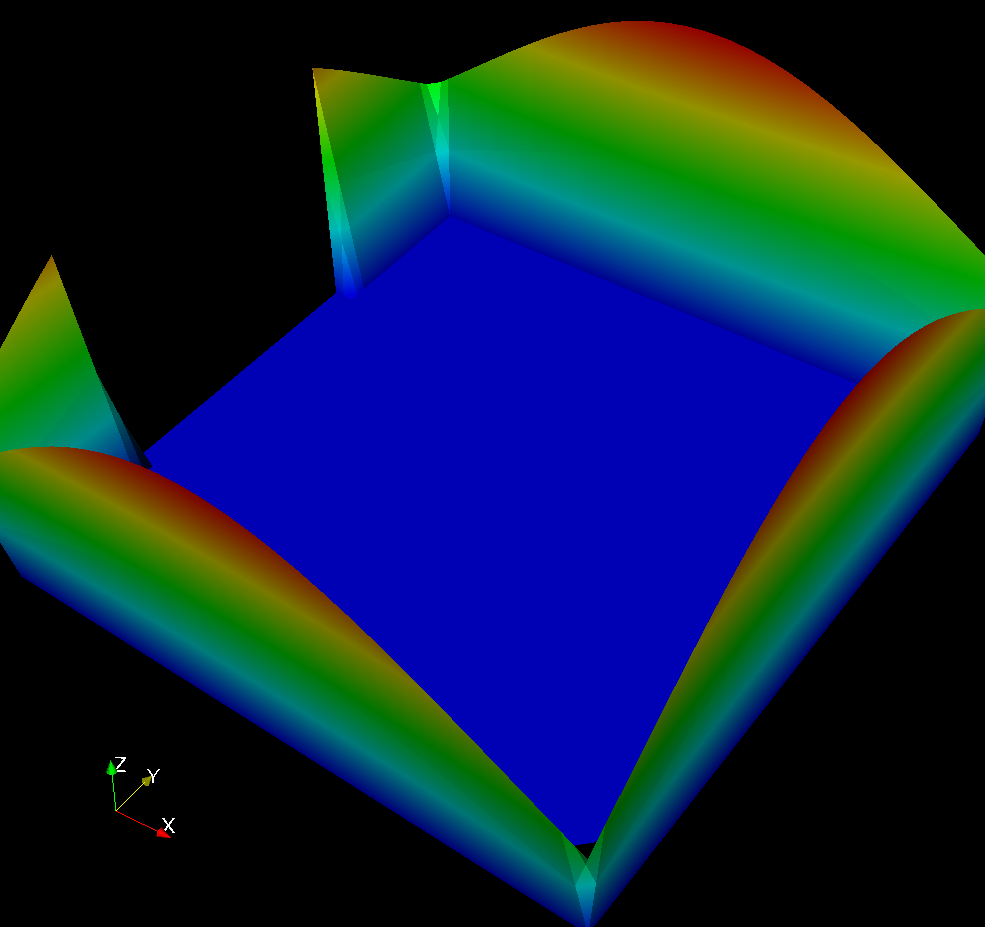
\includegraphics[width=0.65\textwidth]{./EPS/q1constrainedinterpolate}
\end{center}
\end{frame}

Figure \ref{fig:Q1ConstrainedInterpolation} shows the result obtained
after setting the nonconstrained degrees of freedom to zero.


\mode<article>{
\begin{figure}
\begin{center}
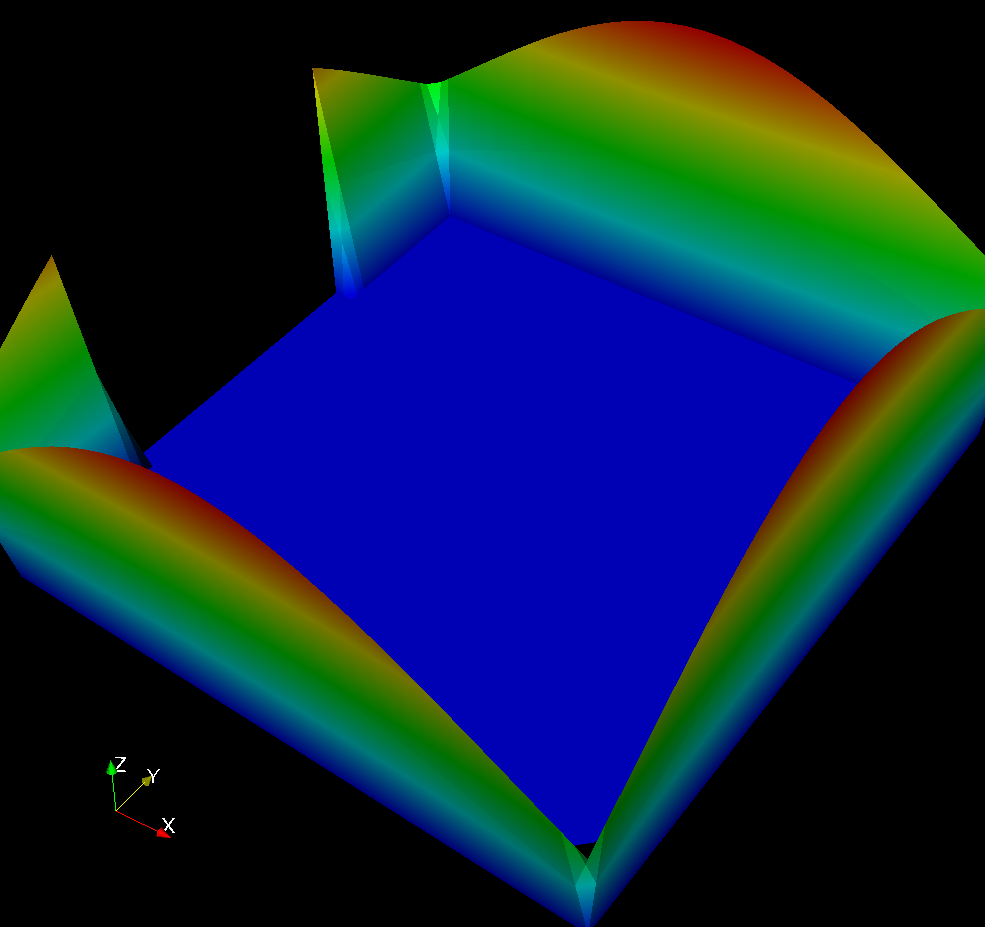
\includegraphics[width=0.5\textwidth]{./EPS/q1constrainedinterpolate}
\end{center}
\caption{Interpolation of $\exp(-3\|x-c\|^2)$ with $Q_1$ elements with
subsequent modification of nonconstrained degrees of freedom.}
\label{fig:Q1ConstrainedInterpolation}
\end{figure}
}

\subsection{Composite Finite Element Spaces}

\mode<article>{
\begin{figure}
\begin{center}
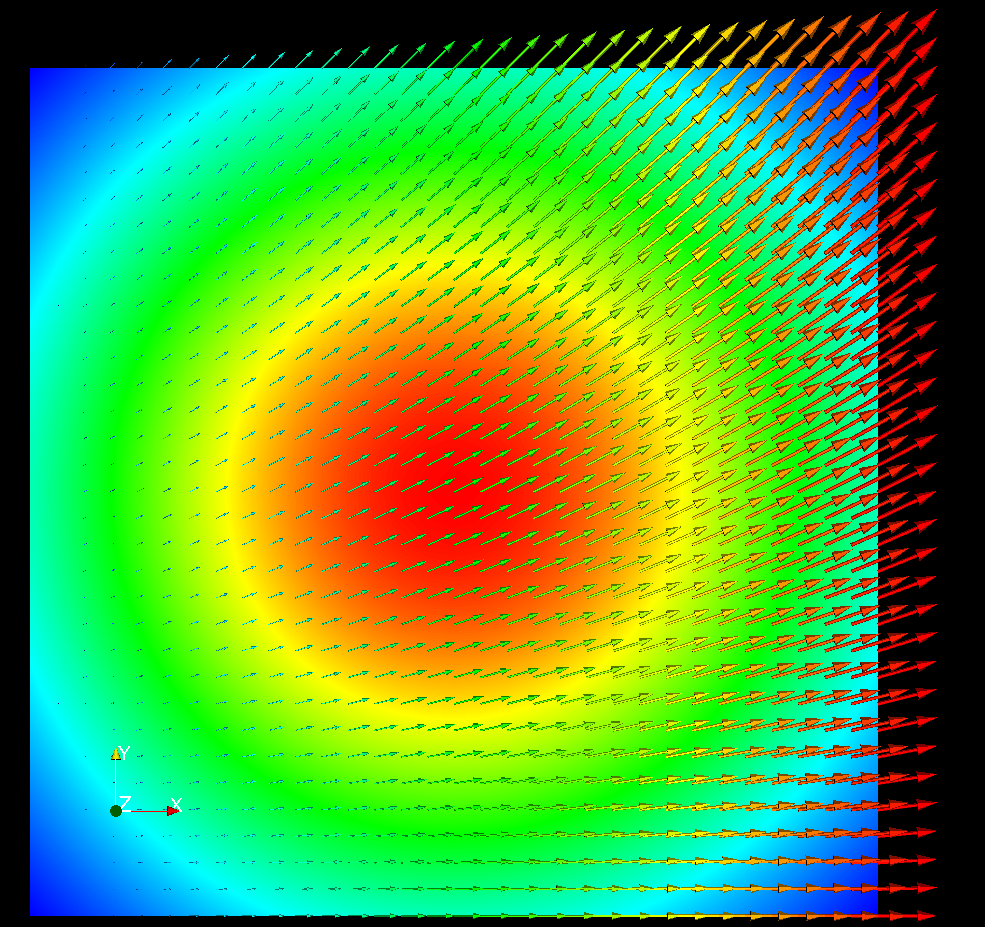
\includegraphics[width=0.5\textwidth]{./EPS/thinterpolate}
\end{center}
\caption{Visualization of velocity field and pressure in the
Taylor-Hood example.}
\label{fig:THInterpolation}
\end{figure}
}

\begin{frame}
\frametitle<presentation>{Composition of Finite Element Spaces}
For systems of PDEs we need product function spaces.

This can be achieved now in a completely generic way:
\begin{itemize}
\item \lstinline{Dune::PDELab::PowerGridFunctionSpace<GFS,k,M>} builds a
new grid function space that is \lstinline{k}-times the product of \lstinline{GFS}.
\item \lstinline{D...::CompositeGridFunctionSpace<M,GFS0,...,GFS8>}
builds a new grid function space out of up to 9 existing grid function
spaces. 
\item \lstinline{M} controls construction of local to global map.
\end{itemize}

This can be applied recursively leading to a type tree.

The local function space reflects this type tree.

\lstinline{Dune::PDELab::GridFunctionSubSpace} allows the selection of
subspaces.

Functions can be composed in a similar way.
\end{frame}

\begin{frame}
\frametitle<presentation>{Taylor-Hood Example}
We now do the Taylor-Hood function space as an example.

As before, we construct the function space and interpolate a finite
element function from a given analytic function.

Let us start by defining a vector-valued analytic function for the
velocity field.  
\end{frame}

\begin{frame}<presentation>[fragile,allowframebreaks,allowdisplaybreaks]
\frametitle<presentation>{Analytic Velocity Field Listing}
\framesubtitle<presentation>{File \texttt{examples/thvelocity.hh}}
\lstinputlisting[basicstyle=\ttfamily\scriptsize,numbers=left, 
numberstyle=\tiny, numbersep=5pt]{../../examples/thvelocity.hh}
\end{frame}
\mode<article>{
\begin{Lst}[File examples/thvelocity.hh] \mbox
\nopagebreak
\lstinputlisting[basicstyle=\ttfamily\scriptsize,numbers=left, 
numberstyle=\tiny, numbersep=5pt]{../../examples/thvelocity.hh}
\end{Lst}}

Now the Taylor-Hood interpolation example.

\begin{frame}<presentation>[fragile,allowframebreaks,allowdisplaybreaks]
\frametitle<presentation>{Taylor Hood Example Listing}
\framesubtitle<presentation>{File \texttt{examples/thinterpolate.hh}}
\lstinputlisting[basicstyle=\ttfamily\scriptsize,numbers=left, 
numberstyle=\tiny, numbersep=5pt]{../../examples/thinterpolate.hh}
\end{frame}
\mode<article>{
\begin{Lst}[File examples/thinterpolate.hh] \mbox
\nopagebreak
\lstinputlisting[basicstyle=\ttfamily\scriptsize,numbers=left, 
numberstyle=\tiny, numbersep=5pt]{../../examples/thinterpolate.hh}
\end{Lst}}

\begin{frame}<presentation>
\frametitle<presentation>{Visualization of Taylor-Hood Function}
\begin{center}
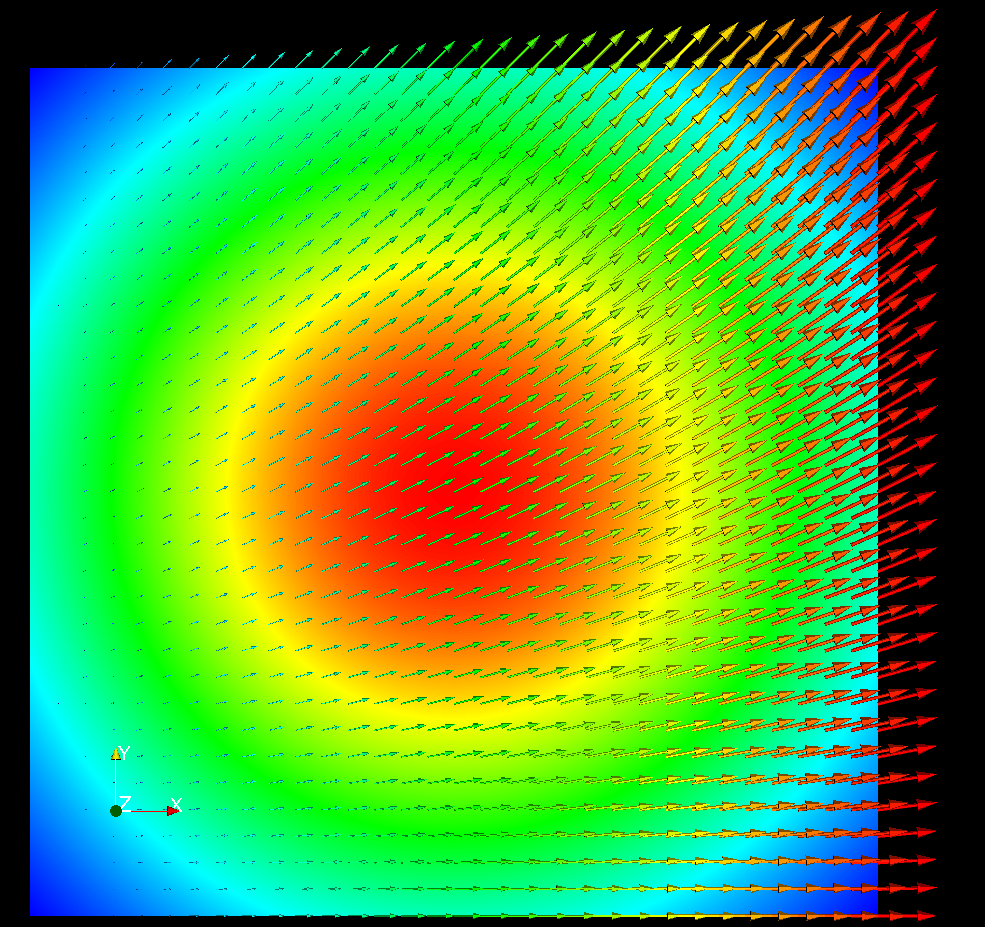
\includegraphics[width=0.5\textwidth]{./EPS/thinterpolate}
\end{center}
\end{frame}

Figure \ref{fig:THInterpolation} visualizes the result of this
example.

\subsection{Summary}

\begin{frame}
\frametitle<presentation>{Function Space Summary}
In order to incorporate a function space in PDELab do the following: 
\begin{itemize}
\item Hope that somebody already included the local basis
in \texttt{dune-localfunctions} and provided the finite element map
in \texttt{dune-pdelab}. 
\item If not, you have to
\begin{itemize}
\item Make a local basis.
\item Make local coefficients.
\item Make a local interpolation.
\item Make a finite element.
\item Make a finite element map.
\end{itemize}
\item Write a constraints assembler if required.
\item Set up the function space via \texttt{GridFunctionSpace}
\end{itemize}
\end{frame}

\cleardoublepage
